\documentclass{standalone}
\usepackage{pgf}
\usepackage{amsmath}
\usepackage{tikz}
\usetikzlibrary{shapes,arrows}
\usetikzlibrary{positioning}
\begin{document}
   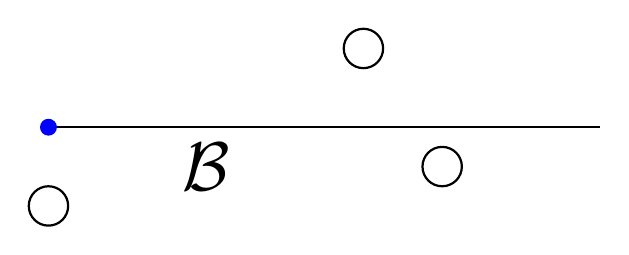
\begin{tikzpicture}
\coordinate  (a) at (-2,-1);
\coordinate  (b) at (3,-0.5);
\coordinate  (c) at (2,1);
 
\draw[thick] (a) circle (0.25cm);
%\node (a) {\Large $\mathcal{R}_1$};

\draw[thick] (b) circle (0.25cm);
%\node (b) {\Large $\mathcal{R}_2$};

\draw[thick] (c) circle (0.25cm);
%\node (c) { $\mathcal{R}_3$};

\draw[thick] (-2,0) -- (+5,0);
  \node[draw=none,align=left] at (0,-0.5) {\Huge $\mathcal{B}$};

\draw[blue,fill=blue] (-2,0) circle (.1cm); 
\end{tikzpicture}
\end{document}

